The proposal of the final TRITIUM monitor is presented in this section. A schematic design is shown in Figure \ref{fig:TritiumDetectorSchematicDesign}. This proposal consists of a number of TRITIUM modules read out in parallel. The design of the modules will be made according to the results obtained from the prototypes. These monitor is shielded from the environmental radioactivity by three different techniques:

\begin{enumerate}

\item{} An external lead shield that stops the environmental radioactivity and soft cosmic rays (particles with energies below $200~\MeV$).

\item{} Several active vetos which are placed below and above the TRITIUM detector. These active vetos are read out in anticoincidence to mitigate high energy background, mainly cosmic ray particles with energies above $200~\MeV$.

\item{} A water purification system which eliminates radioactive elements present in the water samples measured by the TRITIUM monitor.

\end{enumerate}

\begin{figure}[h]
\centering
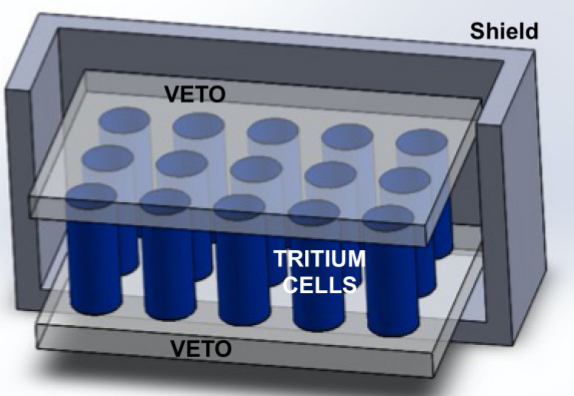
\includegraphics[scale=0.5]{5Prototypes/55ModularTritiumDetector/FinalTritium.png}
\caption{A schematic design of the TRITIUM detector.\label{fig:TritiumDetectorSchematicDesign}}
\end{figure}

The water purification system, the lead shield and a TRITIUM-Aveiro prototype are currently in operation at the Arrocampo site. Furthermore, two additional TRITIUM-Aveiro prototypes and four active vetos currently under construction will be installed in parallel with this prototype. The electronics of the TRITIUM-Aveiro prototype is based on a RaspberryPi and cannot read more than one module due to hardware limitation. A FPGA-based counter board will replace this electronics.

Three TRITIUM-IFIC-2 prototypes and two active veto are already built and will be installed at Arrocampo as soon as possible. At present, lateral cosmic vetos for the TRITIUM-IFIC-2 modules are not foreseen since the influence of side cosmic rays is expected to be small ($\propto \text{cos}^2(\theta)$), but they can be included in the future if necessary.

One of the most important aspects of the TRITIUM monitor is its modular design, which allows scalability to reach the required sensitivity of $100~\becquerel/\liter$. It means that if this target sensitivity is not achieved with three modules, it can be obtained by installing additional modules. The only scalability restriction is the available space which is set by the lead shield and the cabin in which the setup is installed. In the currently available space, five different structures as the one shown in Figure \ref{fig:TritiumMonitorIFIC2Design} can be placed, each containing 10 modules and two active veto. If 50 TRITIUM modules are installed, the sensitivity of the TRITIUM monitor could be improved by a factor of around $\sqrt{50}$ with respect to the sensitivity of a single module.

\begin{figure}[h]
\centering
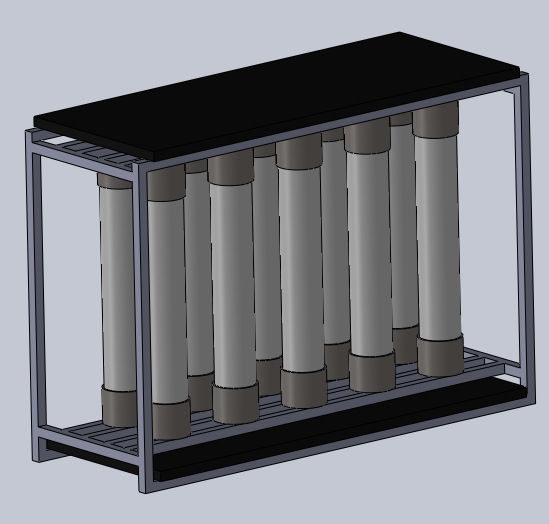
\includegraphics[scale=0.6]{5Prototypes/55ModularTritiumDetector/Tritium_Detector_Based_On_Tritium_IFIC_2.PNG}
\caption{A TRITIUM monitor design based on the TRITIUM-IFIC-2 prototype.\label{fig:TritiumMonitorIFIC2Design}}
\end{figure}